\usepackage{tikz}

\newlength{\offset}

\title{ICS0026 Cryptography}
\subtitle{Certificate validity, eIDAS \& qualified signatures}
\date{\today}
\author{Taaniel Kraavi}
\institute%
{%
  \textit{IT College}\\
  \textit{Tallinn University of Technology}
}

\begin{document}
\begin{frame}
  \titlepage
\end{frame}

\begin{frame}{Refresher on PKI}
  Hierarchical trust model:
  \begin{itemize}[<+(1)->]
    \item Root CA self-signs their own root certificate(s) (trust-anchor)
    \item Root certificates used to certify subordinate/intermediate certificates
    \item Subordinates issue end-entity certificates or certify other subordinates
  \end{itemize}

  \vspace*{1em}

  \pause
  A root certificate is linked to end-entity certificates through intermediate certificates.
  \begin{itemize}[<+(1)->]
    \item This forms the certificate chain
  \end{itemize}

  \vspace*{1em}

  \pause
  Two main authorities:
  \begin{itemize}[<+(1)->]
    \item Certification Authority (CA): issues \& manages certificates
    \item Registration Authority (RA): verifies applicant identities
  \end{itemize}
\end{frame}

\begin{frame}{Getting certificates}
  \pause
  Certificate signing request (CSR):
  \begin{itemize}[<+(1)->]
    \item Apply for a certificate with a CA
    \item Must include significant information (identity data and public key)
    \item Self-signed using applicant's private key (\href{https://datatracker.ietf.org/doc/html/rfc2986}{PKCS \#10})
    \item CA interacts with RA and forwards it the CSR
    \item CA returns CA-signed certificate if RA approves the applicant
  \end{itemize}

  \vspace*{1em}

  \pause
  Other methods exist
  \begin{itemize}[<+(1)->]
    \item Certificate Management Protocol (CMP)
    \item Simple Certificate Enrolment Protocol (SCEP)
  \end{itemize}
\end{frame}

\begin{frame}{X.509 certificates}
  \pause
  Bind a public key to an identity using a digital signature.
  \begin{itemize}[<+(1)->]
    \item \href{https://www.itu.int/rec/T-REC-X.509}{ITU-T X.509}
    \item \enquote{For the Internet}: \href{https://datatracker.ietf.org/doc/html/rfc5280}{RFC 5280}
    \item \href{https://cabforum.org}{CA/Browser Forum certificate baselines}
    \item Self-signed or signed by a CA
    \item ASN.1 structures
  \end{itemize}
\end{frame}

\begin{frame}{X.509 v3}
  Structure:
  \begin{itemize}[<+(1)->]
    \item Certificate
    \begin{itemize}
      \item Version \& serial number
      \item Issuer Name
      \item Subject name
      \item Validity period: not before \& not after
      \item Subject Public Key Info: algorithm \& public key
      \item Signature Algorithm ID
      \item Issuer and/or Subject Unique Identifier (optional)
      \item Extensions (optional)
    \end{itemize}
    \item Certificate Signature Algorithm
    \item Certificate Signature
  \end{itemize}

  \pause
  The above structure is simplified and reordered.
\end{frame}

\begin{frame}{Certificate extensions}
  Certificate extensions:
  \begin{itemize}[<+(1)->]
    \item Uniquely identified by an Object Identifier (OID)
    \item Labelled \enquote{critical} or \enquote{non-critical}
    \begin{itemize}
      \item Must reject certificate if unrecognised critical extension
      \item May ignore an unrecognised non-critical extension
      \item Must process extensions if recognised
    \end{itemize}
    \item Contain a set of values
  \end{itemize}

  \pause
  Restrict usage for specific purposes
  \begin{itemize}[<+(1)->]
    \item All restrictions must be satisfied
    \item Downgrade attacks might be possible
  \end{itemize}
\end{frame}

\begin{frame}{Certificate extensions}
  Some examples:
  \begin{itemize}[<+(1)->]
    \item Basic constraints
    \begin{itemize}
      \item Whether the subject is a CA
      \item Maximal certification path depth
    \end{itemize}
    \item Key usage
    \begin{itemize}
      \item Allowed cryptographic operations
      \item E.g. certificate signing only
    \end{itemize}
    \item Extended Key Usage
    \begin{itemize}
      \item Fine-tune key usage, e.g. only allowed for email
      \item Must not conflict with key usage
    \end{itemize}
    \item \dots
  \end{itemize}
\end{frame}

\begin{frame}{Certificate validity}
  \pause
  Certificate path validation (\href{https://datatracker.ietf.org/doc/html/rfc5280}{RFC 5280} for X.509):
  \begin{itemize}[<+(1)->]
    \item Start from the leaf certificate
    \item Check certificate validity time against current time
    \item Check revocation status (not blacklisted/cancelled)
    \item Verify constraints (e.g. name and policy) and extensions
    \begin{itemize}
      \item Is the chain \enquote{approved}? (subordinate cert approved by parent)
      \item Are all intermediate certificates CA certificates? (no end-entities allowed)
      \item Are CAs allowed to sign subordinate certificates? (approval for delegation)
      \item \dots
    \end{itemize}
    \item Successful only if all checks pass for all nodes until the root
  \end{itemize}

  \pause
  Very tricky, do not implement yourself!
\end{frame}

\begin{frame}{Certification Revocation Lists (CRL)}
  List of \emph{unexpired} certificates revoked by a CA:
  \begin{itemize}[<+(1)->]
    \item Two states: revoked (definitive) \& hold (might be reinstated)
    \begin{itemize}
      \item Revocation reason optional
    \end{itemize}
    \item List must be periodically published by the CA
    \begin{itemize}
      \item Can be delegated to another trusted and authorised authority
      \item Signed by the publisher
      \item Lifetime? (e.g. CA/Browser Forum requirements)
    \end{itemize}
    \item Certificate field: CRL Distribution Points
    \item \emph{Relying party} must parse the entire list
  \end{itemize}
\end{frame}

\begin{frame}{Liability and CRLs}
  \pause
  Who is liable during the \enquote{grace period}?
  \begin{itemize}[<+(1)->]
    \item Certificate revoked but not in the public CRL yet
    \item Complex question with no clear laws/answers
  \end{itemize}

  \pause
  Revocation should be checked before use for critical certs
  \begin{itemize}[<+(1)->]
    \item Danger: DoS attacks
    \item Browsers do not do it for leaf certs\textsuperscript{*}
    \item Browsers use mechanisms for validating intermediate certs
  \end{itemize}
\end{frame}

\begin{frame}{Online Certificate Status Protocol (OCSP)}
  Online Certificate Status Protocol (OCSP):
  \begin{itemize}[<+(1)->]
    \item \href{https://datatracker.ietf.org/doc/html/rfc6960}{RFC 6960}
    \item Protocol to obtain the revocation status of a certificate
    \item OCSP \emph{responders}: endpoints for OCSP requests
    \item Responders: either CA or CA-authorised (delegated) responders
    \item Certificate field: Authority Information Access
    \item OCSP response status: \enquote{good}, \enquote{revoked}, \enquote{unknown}
  \end{itemize}
\end{frame}

\begin{frame}{OCSP vs. CRL}
  \begin{itemize}[<+(1)->]
    \item Responses are concrete and small: better for clients to parse
    \item Cheaper for clients, but expensive for CAs
    \item Asserts the validity at the specific time\textsuperscript{*}
    \begin{itemize}
      \item Trip delay error margin
      \item Caching of OCSP responses
    \end{itemize}
    \item DoS possible for both
  \end{itemize}
\end{frame}

\begin{frame}{Issues with OCSP}  
  \pause
  Replay attacks:
  \begin{itemize}[<+(1)->]
    \item For efficiency, OCSP responses are often pre-signed
    \item Check the OCSP issuing time (thisUpdate \& nextUpdate fields)
    \item OCSP nonce extension: random nonce for the request
  \end{itemize}

  \pause
  Privacy concerns:
  \begin{itemize}[<+(1)->]
    \item Requires third-party contact
    \item Leaks query information (e.g. websites browsed)
  \end{itemize}
\end{frame}

\begin{frame}{OCSP stapling}
  \pause
  Include an OCSP response with the data responses:
  \begin{itemize}[<+(1)->]
    \item Server periodically makes OCSP requests to the CA itself
    \item Server sends the requests back with the requested data
    \item OCSP response still signed by the responder
    \item E.g. website serving the OCSP response alongside the HTTPS certificates
  \end{itemize}

  \pause
  Formally known as the \enquote{TLS Certificate Status Request} extension.
\end{frame}

\begin{frame}{OCSP stapling}
  \begin{figure}
    \centering
    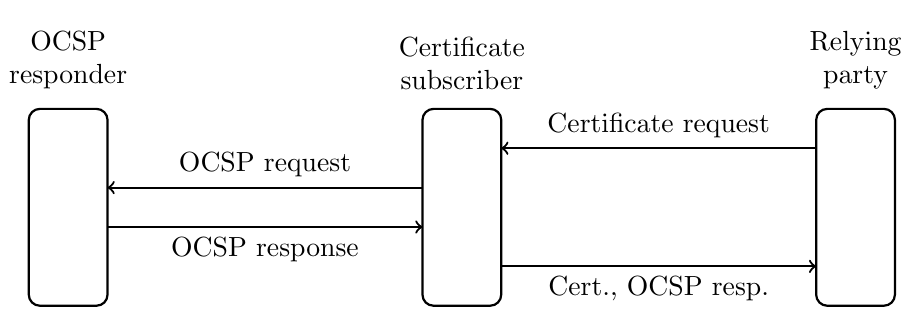
\begin{tikzpicture}
      \draw[rounded corners,thick] (0, 0) rectangle  ++(1,-2.5);
      \draw[rounded corners,thick] (5, 0) rectangle ++(1,-2.5);
      \draw[rounded corners,thick] (10, 0) rectangle ++(1,-2.5);

      \node[label={[align=center]Certificate\\subscriber}] at (5.5, 0) {};

      % Set the picture size to everything drawn so far.
      % This ignores the label sizes for centering.
      \useasboundingbox (current bounding box);
    
      \node[label={[align=center]OCSP\\responder}] at (0.5, 0) {};
      \node[label={[align=center]Relying\\party}] at (10.5, 0) {};
    
      \draw[<-,thick] (6, -0.5) -- (10, -0.5) node[midway,above] {Certificate request};
      \draw[<-,thick] (1, -1) -- (5, -1) node[midway,above] {OCSP request};
      \draw[->,thick] (1, -1.5) -- (5, -1.5) node[midway,below] {OCSP response};
      \draw[->,thick] (6, -2) -- (10, -2) node[midway,below] {Cert., OCSP resp.};
    \end{tikzpicture}
  \end{figure}
\end{frame}

\begin{frame}{Missing staple}
  \pause
  What to do if the cert is not stapled?
  \begin{itemize}[<+(1)->]
    \item Query the responder directly
    \item What if an attacker drops the requests?
  \end{itemize}
  
  \pause
  OCSP must staple extension
  \begin{itemize}[<+(1)->]
    \item Fail the task if no OCSP response provided
    \item Prevents some downgrade attacks
  \end{itemize}

  \pause
  CAs do not typically like OCSP, and stapling is not very popular
\end{frame}

\begin{frame}{TLS Certificate Status Request}
  OCSP and TLS:
  \begin{itemize}[<+(1)->]
    \pause \item \href{https://datatracker.ietf.org/doc/html/rfc6066}{RFC 6066}: TLS extensions
    \begin{itemize}
      \item For TLS 1.2 only a single OCSP response could be sent
      \item Cert chain cannot thus be validated
      \item \href{https://datatracker.ietf.org/doc/html/rfc6961}{RFC 6961} added support for multiple responses
    \end{itemize}
    \pause \item \href{https://datatracker.ietf.org/doc/html/rfc8446}{RFC 8446}: TLS 1.3
    \begin{itemize}
      \item Fixes the single OCSP-response problem of TLS 1.2
      \item Obsoletes RFC 6961
    \end{itemize}
  \end{itemize}
\end{frame}

\begin{frame}{Disclaimer}
  Everything that follows is grossly oversimplified.
  \pause
  \begin{itemize}
    \item Legal rather than cryptographic topics
    \item Numerical identity vs. legal identity
    \item Laws attach legal validity to technical validity
  \end{itemize}
\end{frame}

\begin{frame}{eIDAS}
  Electronic Identification, Authentication and Trust Services
  \begin{itemize}[<+(1)->]
    \item EU regulation: directly applicable to all member states
    \item Interoperability of electronic identification (eID) \& trust services
    \item Legal validity
    \item National identity providers (IdP)
  \end{itemize}

  \vfill

  \pause
  eIDAS \enquote{2.0} amends the original regulation.
  \begin{itemize}[<+(1)->]
    \item \href{https://eur-lex.europa.eu/eli/reg/2024/1183/oj}{Regulation (EU) 2024/1183}
    \item Introduces digital identity wallets
    \item The amendments are out of our scope
  \end{itemize}
\end{frame}

\begin{frame}{eIDAS eID}
  eIDAS eID online service access:
  \begin{enumerate}[<+(1)->]
    \item A citizen requests an on-line service in another Member State.
    \item The citizen is requested to authenticate themselves by the on-line service.
    \item The citizen chooses to authenticate with an eIDAS eID.
    \item The authentication request is sent to the citizen's country for authentication.
    \item The authentication result is returned to the service provider.
    \item Authentication is complete and the citizen can proceed.
  \end{enumerate}

  \pause
  {\scriptsize Source: \href{https://ec.europa.eu/digital-building-blocks/sites/display/DIGITAL/eID}{\textit{Digital Europe Programme eID FAQ}}}

  \pause
  See also: \href{https://www.eid.as/tsp-map/}{eIDAS eID map}
\end{frame}

\begin{frame}{Trust services}
  Electronic services that help various parties make \emph{binding} decisions.
  \begin{itemize}[<+(1)->]
    \item Timestamping
    \item E-signing
    \item Digital authentication
    \item Validity confirmation
    \item \dots
  \end{itemize}

  \pause
  EU/EEA Trusted List Browser
  \begin{itemize}[<+(1)->]
    \item Qualified status granted by supervisory body
    \item Member states maintain their own trusted lists
    \item EU maintains the list of trusted lists (EU-level PKI)
    \item {\scriptsize \url{https://eidas.ec.europa.eu/efda/tl-browser/}}
    \item {\scriptsize \url{https://ec.europa.eu/tools/lotl/eu-lotl.xml}}
  \end{itemize}
\end{frame}

\begin{frame}{eIDAS signature levels}
  Article 3:
  \settowidth{\offset}{10}
  \addtolength{\leftmargini}{\offset}
  \begin{itemize}[<+(1)->]
    \item[(10)] \enquote{electronic signature (ES)}
    \item[(11)] \enquote{advanced electronic signature (AdES)}
    \item[(12)] \enquote{qualified electronic signature (QES)}
  \end{itemize}
\end{frame}

\begin{frame}{Electronic signature (ES)}
  \enquote{electronic signature (ES)} means data in electronic form which is attached to or logically associated with other data in electronic form and which is used by the signatory to sign;
\end{frame}

\begin{frame}{Advanced electronic signature (AdES)}
  \enquote{advanced electronic signature (AdES)} means an electronic signature which meets the requirements set out in Article 26;
  \settowidth{\offset}{26.1}
  \addtolength{\leftmargini}{\offset}
  \begin{enumerate}[<+(1)->]
    \item[(26.a)] it is uniquely linked to the signatory;
    \item[(26.b)] it is capable of identifying the signatory;
    \item[(26.c)] it is created [\dots] under his sole control; and
    \item[(26.d)] [\dots] any subsequent change in the data is detectable.
  \end{enumerate}
\end{frame}

\begin{frame}{Qualified electronic signature (QES)}
  \enquote{qualified electronic signature (QES)} means an \emph{advanced electronic signature} that is created by a \emph{qualified electronic signature creation device}, and which is based on a \emph{qualified certificate} for electronic signatures;
  \begin{itemize}[<+(1)->]
    \item qualified certificate: certificate issued by a qualified trust service provider
  \end{itemize}

  \vfill

  \pause
  AdES/QC: advanced electronic signature (AdES) based on a qualified certificate.
\end{frame}

\begin{frame}{Signature levels simplified}
  \pause
  Electronic signatures (ES):
  \begin{itemize}[<+(1)->]
    \item Data used by a signatory to express signing \emph{intent}
    \item E.g. signing an email with your name
  \end{itemize}

  \pause
  Advanced electronic signature (AdES):
  \begin{itemize}[<+(1)->]
    \item Electronic signature \emph{uniquely} linked to an \emph{identifiable} entity
    \item Must assert the \emph{integrity} of signed data
    \item E.g. signature issued with OpenSSL for a published certificate
    \item If the certificate is qualified: AdES/QC
  \end{itemize}

  \pause
  Qualified electronic signature
  \begin{itemize}[<+(1)->]
    \item AdES where the certificate and signing device are qualified
    \item E.g. digital signatures issued with an Estonian ID card
  \end{itemize}
\end{frame}

\begin{frame}{Qualified Signature Creation Devices (QSCD)}
  \pause
  eIDAS Annex II:
  \settowidth{\offset}{1.a}
  \addtolength{\leftmargini}{\offset}
  \begin{enumerate}[<+(1)->]
    \item[(1.a)] the confidentiality of the electronic signature creation data [\dots] is reasonably assured;
    \item[(1.b)] the [\dots] data [\dots] can practically occur only once;
    \item[(1.c)] the [\dots] data [\dots] cannot [\dots] be derived and the electronic signature is reliably protected against forgery [\dots];
    \item[(1.d)] the [\dots] data [\dots] can be reliably protected by the legitimate signatory against use by others.
  \end{enumerate}

  \pause
  TL;DR: It should only be possible to issue signatures when possessing the device, and its use should be restricted (e.g. protected by a PIN).
\end{frame}

\begin{frame}{Validating Qualified Electronic Sigantures}
  How to validate QES signatures?
  \begin{itemize}[<+(1)->]
    \item \href{https://eur-lex.europa.eu/legal-content/EN/TXT/HTML/?uri=CELEX\%3A32014R0910\#d1e2594-73-1}{Article 32}
    \item Quite tricky!
  \end{itemize}

  \pause
  Qualified Validation Service:
  \begin{itemize}
    \item \href{https://eur-lex.europa.eu/legal-content/EN/TXT/HTML/?uri=CELEX:32014R0910\#d1e2664-73-1}{Article 33}
    \item Automated validation process
    \item Use over self-implementation whenever possible
    \begin{itemize}
      \item If nothing else, check for libraries
    \end{itemize}
  \end{itemize}

  \pause
  (\href{https://eur-lex.europa.eu/legal-content/EN/TXT/HTML/?uri=OJ:L\_202401183\#d1e3370-1-1}{\textit{eIDAS 2.0 amendments}})
\end{frame}

\begin{frame}{Trusted timestamping}
  \pause
  Article 3:
  \settowidth{\offset}{33}
  \addtolength{\leftmargini}{\offset}
  \begin{enumerate}
    \item[(33)] \enquote{electronic time stamp} means data in electronic form which binds other data in electronic form to a particular time establishing evidence that the latter data existed at that time;
  \end{enumerate}

  \pause
  Article 41:
  \begin{itemize}
    \setcounter{enumi}{1}
    \item A qualified electronic time stamp shall enjoy the presumption of the accuracy of the date and the time it indicates and the integrity of the data to which the date and time are bound.
  \end{itemize}
\end{frame}

\begin{frame}{Trusted timestamping}
  \pause
  Signed statement by a Time Stamping Authority (TSA):
  \begin{itemize}[<+(1)->]
    \item TSAs must use an accurate time source
    \item TSAs must log issued timestamps
  \end{itemize}

  \pause
  \href{https://datatracker.ietf.org/doc/html/rfc3161}{RFC 3161}:
  \begin{itemize}[<+(1)->]
    \item Internet X.509 Public Key Infrastructure Time-Stamp Protocol
  \end{itemize}

  \pause
  Time does not exist in cryptography:
  \begin{itemize}[<+(1)->]
    \item Relative temporal ordering is the best we can achieve
    \begin{itemize}
      \item E.g. which document was signed earlier (earlier in a chain)
    \end{itemize}
    \item Even chain-based TSAs require \enquote{trust} (e.g. Guardtime)
  \end{itemize}
\end{frame}

\begin{frame}{Legal effects of electronic signatures}
  \pause
  Article 25:
  \begin{enumerate}
    \setcounter{enumi}{1}
    \item A qualified electronic signature shall have the equivalent legal effect of a handwritten signature.
  \end{enumerate}

  \vspace*{1em}

  \pause
  Legal implication:
  \begin{itemize}[<+(1)->]
    \item Accusing party needs not prove that an entity issued the signature.
    \item Issuer has to prove that they did not issue the signature.
    \item $\implies$ legal non-repudiation
    \item Article 13, paragraph 1
  \end{itemize}
\end{frame}

\begin{frame}{Digital vs. electronic signature}
  Digital signature:
  \begin{itemize}[<+(1)->]
    \item Cryptographic concept
    \item A tool to prove integrity and provenance
  \end{itemize}

  \vspace*{1em}

  \pause
  Electronic signature:
  \begin{itemize}[<+(1)->]
    \item Legal concept defined in eIDAS
    \item Signature on some data: intent of signatory to associate with this data
    \item Not necessarily cryptographic (e.g. name on an email)
  \end{itemize}

  \vspace*{1em}

  \pause
  Not all electronic signatures are digital signatures!
\end{frame}

\begin{frame}{ETSI signature standards (eIDAS versions)}
  ETSI specifies three formats for AdES+\dots
  \begin{itemize}[<+(1)->]
    \item XML advanced electronic signature (XAdES)
    \begin{itemize}
      \item \href{http://www.etsi.org/deliver/etsi_ts/103100_103199/103171/02.01.01_60/ts_103171v020101p.pdf}{ETSI TS 103 171 v.2.1.1}
    \end{itemize}
    \item CMS advanced electronic signature (CAdES)
    \begin{itemize}
      \item \href{http://www.etsi.org/deliver/etsi_ts/103100_103199/103173/02.02.01_60/ts_103173v020201p.pdf}{ETSI TS 103 173 v.2.2.1}
    \end{itemize}
    \item PDF advanced electronic signature (PAdES)
    \begin{itemize}
      \item \href{http://www.etsi.org/deliver/etsi_ts/103100_103199/103172/02.02.02_60/ts_103172v020202p.pdf}{ETSI TS 103 172 v.2.2.2}
    \end{itemize}
  \end{itemize}

  \pause
  \dots and one container format
  \pause
  \begin{itemize}
    \item Associated Signature Container (ASiC)
    \item \href{http://www.etsi.org/deliver/etsi_ts/103100_103199/103174/02.02.01_60/ts_103174v020201p.pdf}{ETSI TS 103 174 v.2.2.1}
  \end{itemize}
\end{frame}

\begin{frame}{ETSI conformance levels}
  \pause
  Incremental requirements for long-term signature validity:
  \begin{enumerate}[<+(1)->]
    \item B-B: valid until the signature certificate is valid
    \begin{itemize}
      \item \enquote{Short-term} signatures
    \end{itemize}
    \item B-T: prove that the signature existed at a certain time
    \begin{itemize}
      \item Trusted token: TSA-signed time-stamp and signature digest
    \end{itemize}
    \item B-LT: long-term availability of validation material
    \begin{itemize}
      \item Include also the OCSP/CLR status + chain at the time
    \end{itemize}
    \item B-LTA: long-term availability and integrity of validation material
    \begin{itemize}
      \item Include a \enquote{document-time-stamp} token
      \item Encompasses also the validation material
      \item Tokens can be subsequently added to prolong validity
    \end{itemize}
  \end{enumerate}
\end{frame}

\begin{frame}{XAdES}
  XML advanced electronic signature
  \begin{itemize}[<+(1)->]
    \item Based on XML digital signatures (XMLDSig)
    \item W3C recommendation: XML Signature Syntax and Processing
    \item Human and machine readable
    \item Signs any document/data (including binary data)
    \item Can sign multiple files with one signature
  \end{itemize}    
\end{frame}

\begin{frame}{CAdES}
  CMS advanced electronic signature
    \begin{itemize}[<+(1)->]
      \item Cryptographic Message Syntax (CMS)
      \item Signs only binary data, signatures not human readable
      \item Lacks XAdES features (e.g. multi-document signing), and offers none more
    \end{itemize}
\end{frame}

\begin{frame}{PAdES}
  PDF advanced electronic signature
  \begin{itemize}[<+(1)->]
    \item Signatures embedded within the PDF
    \item Included in the ISO PDF standard
    \item Signing and verification included in PDF software\textsuperscript{*}
  \end{itemize}

  \vspace*{1em}

  \pause
  PAdES is much more limited than X/CAdES, but is more \enquote{portable}.
\end{frame}

\begin{frame}{XAdES signing modes}
  Two signing modes:
  \begin{itemize}[<+(1)->]
    \item Detached: data is separate from the signature
    \begin{itemize}
      \item The original data is not modified
    \end{itemize}
    \item Encapsulated: XML file encapsulating the data
    \begin{itemize}
      \item Not usable/practical with all types of data
      \item Signature and data in the same file
    \end{itemize}
  \end{itemize}

  \vspace*{1em}

  \pause
  How to prevent signature/data loss for detached signatures?
\end{frame}

\begin{frame}{Associated Signature Containers (ASiC)}
  Data container grouping data objects with signatures and/or timestamps.
  \begin{itemize}[<+(1)->]
    \item Associates detached signatures with referenced data
    \begin{itemize}
      \item Aims to prevent the loss of signatures/data
      \item Can group signatures of multiple signatories
    \end{itemize}
    \item ZIP format (no compression)
    \item Developed by ETSI
    \begin{itemize}
      \item \href{http://www.etsi.org/deliver/etsi_ts/103100_103199/103174/02.02.01_60/ts_103174v020201p.pdf}{ETSI TS 103 174 V2.2.1 (2013-06)}
      \item \href{http://www.etsi.org/deliver/etsi_en/319100_319199/31916202/01.01.01_60/en_31916202v010101p.pdf}{ETSI EN 319 162-1 V1.1.1 (2016-04)}
    \end{itemize}
    \item 2013 version required by eIDAS
    \item Usable with XAdES and CAdES, but not PAdES
  \end{itemize}
\end{frame}

\begin{frame}{Two types of ASiC}
  Two main types:
  \begin{itemize}[<+(1)->]
    \item Simple (ASiC-S)
    \begin{itemize}
      \item Signature(s) must reference only a single file
    \end{itemize}
    \item Extended (ASiC-E)
    \begin{itemize}
      \item Signature(s) may reference multiple files
      \item Used in Estonia
    \end{itemize}
  \end{itemize}

  \vspace*{1em}

  \pause
  There are more details \& subtleties.
\end{frame}

\begin{frame}{ASiC structure}
  Two folders:
  \begin{itemize}[<+(1)->]
    \item \enquote{root} folder: contains the file and all other content
    \item \texttt{META-INF} folder: contains content metadata and signatures
  \end{itemize}
\end{frame}

\begin{frame}{Estonia and containers}
  A short history/summary of the Estonian digital signature (articles):
  \begin{itemize}
    \item \href{https://www.id.ee/en/article/bdoc2-1-new-estonian-digital-signature-standard-format/}{BDOC2.1 --- New Estonian digital signature standard format}
    \item \href{https://www.id.ee/en/article/digidoc-container-format-life-cycle-2/}{DigiDoc container format life cycle}
  \end{itemize}

  \vspace*{1em}

  \pause
  DigiDoc is the software used in Estonia for interacting with signed and/or encrypted containers.
\end{frame}

\end{document}
